% Website CV. Build from the repository root with:
% pdflatex -interaction=nonstopmode -halt-on-error -output-directory=/tmp/cv-build cv/cv_Phat.tex
% Publication update: 19 November 2026.
% !TEX program = pdflatex
\documentclass[11pt,a4paper]{article}

\usepackage[left=2.25cm,right=2.25cm,top=1.85cm,bottom=1.7cm]{geometry}
\usepackage[T1]{fontenc}
\usepackage{times}
\usepackage{fix-cm}
\usepackage{graphicx}
\usepackage{xcolor}
\usepackage{pict2e}
\usepackage{hyperref}
\usepackage{enumitem}
\usepackage{tabularx}
\usepackage{fancyhdr}
\usepackage{needspace}
\definecolor{linkblue}{HTML}{00A6E8}
\definecolor{rolegray}{HTML}{444444}

\newcommand{\vietnamflag}{%
  \begingroup
  \setlength{\unitlength}{0.8pt}%
  \raisebox{-0.25pt}{%
    \begin{picture}(15,10)
      \put(0,0){\color[HTML]{DA251D}\rule{12pt}{8pt}}%
      \color[HTML]{FFFF00}%
      \polygon*(7.5,8)(8.17,5.93)(10.35,5.93)(8.59,4.65)(9.26,2.57)%
        (7.5,3.85)(5.74,2.57)(6.41,4.65)(4.65,5.93)(6.83,5.93)%
    \end{picture}%
  }%
  \endgroup
}

\hypersetup{colorlinks=true,urlcolor=linkblue,linkcolor=linkblue,pdftitle={Phat Tuan Tran-Truong - Curriculum Vitae},pdfauthor={Phat Tuan Tran-Truong},pdfsubject={Academic CV - updated November 2026}}

\pagestyle{fancy}
\fancyhf{}
\renewcommand{\headrulewidth}{0pt}
\cfoot{\thepage}

% keep bullets and paragraphs from splitting across pages
\clubpenalty=10000
\widowpenalty=10000
\interlinepenalty=10000

\setlength{\parindent}{0pt}
\setlength{\parskip}{0pt}
\setlist[itemize]{leftmargin=1.35em,itemsep=2pt,topsep=3pt,parsep=0pt}

\newcommand{\sectiontitle}[1]{%
  \Needspace{5\baselineskip}
  \vspace{0.28cm}%
  {\Large\bfseries #1}\par\vspace{0.08cm}\hrule\vspace{0.18cm}%
}
\newcommand{\headerline}[2]{%
  \noindent\begin{tabular*}{\textwidth}{@{}l@{\extracolsep{\fill}}r@{}}
  #1 & #2
  \end{tabular*}\par
}
\newcommand{\entry}[4]{%
  \vspace{0.16cm}
  \headerline{\textbf{#1}}{\textbf{#2}}
  {#3}\par
  #4
}
\newcounter{pubcounter}
\newcommand{\pubentry}[2]{%
  \stepcounter{pubcounter}%
  \vspace{0.045cm}
  \noindent\small\linespread{0.97}\selectfont\begin{tabularx}{\textwidth}{@{}p{0.78cm}@{}X@{}}
  [\thepubcounter] & #2
  \end{tabularx}
  \normalsize
}
\newcommand{\rolenote}[1]{%
  \vspace{0.02cm}
  \noindent\small\begin{tabularx}{\textwidth}{@{}p{0.78cm}@{}X@{}}
   & \color{rolegray}\itshape #1
  \end{tabularx}
  \normalsize\vspace{0.05cm}
}
\newcommand{\groupheading}[1]{%
  \Needspace{5\baselineskip}
  \vspace{0.08cm}\par{\small\bfseries #1}\par\vspace{0.01cm}\nopagebreak[4]%
}
\newcommand{\subpubheading}[1]{%
  \Needspace{5\baselineskip}
  \vspace{0.10cm}\par{\bfseries #1}\par\vspace{0.02cm}\nopagebreak[4]%
}
\newcommand{\pubheading}[1]{%
  \Needspace{5\baselineskip}
  \vspace{0.14cm}\par{\bfseries #1}\par\vspace{0.02cm}
}
\newcommand{\awardentry}[2]{%
  \vspace{0.06cm}
  \noindent\begin{tabularx}{\textwidth}{@{}p{2.75cm}X@{}}
  \textbullet\quad #1 & #2
  \end{tabularx}
}
\newcommand{\me}{\underline{\textbf{P. T. Tran-Truong}}}

\newcommand{\refentry}[4]{%
  \vspace{0.16cm}
  \headerline{\textbf{\href{#2}{#1}}}{\small\href{mailto:#4}{#4}}
  {\small #3}\par
}

\begin{document}

\begin{minipage}[t]{0.70\textwidth}
  {\LARGE\bfseries Phat Tuan Tran-Truong (Leo)}\par
  \vspace{0.06cm}
  {\small Legal name on degree certificates: Tran Truong Tuan Phat}\par
  \vspace{0.10cm}
  [\href{https://leotttphat.github.io}{\textcolor{linkblue}{Homepage}}]\quad
  [\href{https://scholar.google.com/citations?user=id3PATEAAAAJ&view_op=list_works&sortby=pubdate}{\textcolor{linkblue}{Google Scholar}}]\quad
  [\href{https://www.linkedin.com/in/tuanphat}{\textcolor{linkblue}{LinkedIn}}]

  \vspace{0.15cm}
  Lecturer and Researcher (M.Eng.)\\
  Faculty of Computer Science \& Engineering, HCMUT, VNU-HCM\nobreak\hspace{0.35em}\vietnamflag

  \vspace{0.12cm}
  Prospective PhD candidate --- Trustworthy AI, Verified and Auditable Agentic Systems, Software/Data Security \& Privacy

  \vspace{0.12cm}
  Email: \href{mailto:phatttt@hcmut.edu.vn}{phatttt@hcmut.edu.vn}\quad
  Mobile: (+84) 368865745\\
  ORCID iD: \href{https://orcid.org/0000-0003-3199-6333}{0000-0003-3199-6333}
\end{minipage}
\hfill
\begin{minipage}[t]{0.24\textwidth}
  \raggedleft
  {\Large\bfseries Curriculum Vitae}\\[0.22cm]
  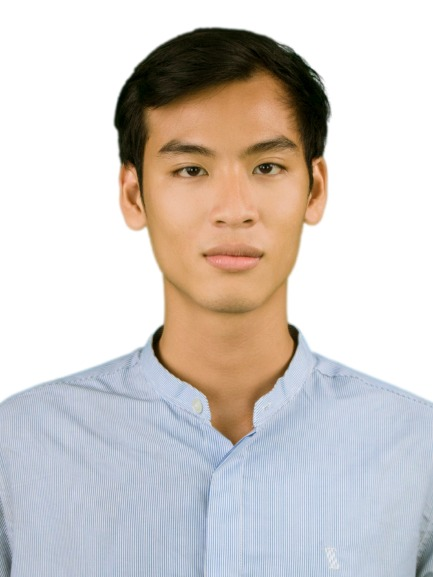
\includegraphics[width=0.78\linewidth]{cv/portrait.jpg}
\end{minipage}

\sectiontitle{Executive Summary}
Lecturer and researcher at HCMUT, VNU-HCM, with an M.Eng.\ by Research in Computer Science and 40+ peer-reviewed papers, including 10+ Q1 journal articles (ESWA, EAAI, MLJ, JNCA, CAEAI, JISA) and 20+ papers across CORE A*/A main-conferences and affiliated tracks/workshops (SIGKDD, ICDM, ASE, EMNLP, EACL, WSDM, WACV, CIKM, ISSRE, ICSOC, ICSA, ESORICS, AsiaCCS). My research focuses on the security and reliability of LLM agent systems, including cross-session memory leakage auditing, reliability estimation, analysis of model-generated code, and capability enforcement. This work builds on experience in differential privacy, privacy-preserving distributed systems, and software supply-chain security. I am seeking a PhD at the intersection of trustworthy AI, software engineering, and security and privacy, with a focus on developing rigorous methods for analysing, evaluating, and securing AI systems.

\sectiontitle{Educational Background}
\entry{2021 -- 2023}{Ho Chi Minh City University of Technology, VNU-HCM}
{M.Eng. by Research in Computer Science}
{\begin{itemize}
  \item CGPA: \textbf{9.05/10}; degree classification \textbf{Very Good}
  \item Thesis: \textbf{Privacy-Preserving Deep Learning Methods}, grade \textbf{9.3/10}
  \item Supervisors: \href{https://scholar.google.com/citations?hl=en&user=3hnmhI4AAAAJ}{Assoc. Prof. Hong Trang Le} and \href{https://scholar.google.com/citations?hl=vi&user=VsxZa7sAAAAJ}{Assoc. Prof. Tran Khanh Dang}
\end{itemize}}

\entry{2016 -- 2020}{Ho Chi Minh City University of Technology, VNU-HCM}
{B.Eng. (Honors) in Computer Science --- degree classification \textbf{Very Good}}
{\begin{itemize}
  \item Thesis: \textbf{Privacy-Preserving Open Data Publishing Based on Data Anonymization}, grade \textbf{9.85/10}
  \item Chief member in the \href{https://sti.vista.gov.vn/projects/kqnv/ky-thuat-an-danh-bao-ve-tinh-rieng-tu-cho-du-lieu-mo-125329.html}{Anonymization Infrastructure for Open Data} project funded by the HCMC Department of Science and Technology.
\end{itemize}}

\sectiontitle{Research Experience}
\entry{Jun 2024 -- present}{Ho Chi Minh City University of Technology, VNU-HCM}
{Lecturer/Researcher, Department of Software Engineering}
{\begin{itemize}
  \item Affiliated with the \href{https://ura.hcmut.edu.vn/}{\textbf{URA Lab}} (led by Assoc. Prof. Tho Quan) and the \href{https://raise-website.vercel.app/}{\textbf{RAISE Lab}} (led by Dr. Xuan-Bach Le); lead researcher for the group's work on \textbf{LLM agent security and reliability}.
  \item \textbf{Formulated} the cross-session leakage threat model for graph-structured agent memory, \textbf{designed} its leakage metric, and \textbf{implemented} the evaluation harness --- accepted at CIKM 2026 (CORE A).
  \item \textbf{Derived} Markov-chain bounds on end-to-end reliability for multi-step agent pipelines and \textbf{implemented} the estimator, replacing case-by-case failure enumeration with a distributional guarantee --- ISSRE 2026 (CORE A).
  \item \textbf{Proposed} treating language models as program samplers so generated code can be analysed distributionally, and \textbf{ran} all experiments --- ASE 2026, NIER track (CORE A*).
  \item \textbf{Designed} a purpose-bound capability model for delegated agent workflows and \textbf{built} its enforcement layer --- SecAssure @ ESORICS 2026.
  \item \textbf{Designed} a hypothesis-to-verification pipeline that turns natural-language hypotheses into verified data-mining discoveries, and \textbf{led} its experimental design --- ICDM 2026 (CORE A*).
  \item \textbf{Direct} the group's malicious-package detection effort; \textbf{contributed} taint-based code slicing and evaluation design to an LLM-based NPM detector --- ARES 2026 Workshops.
  \item \textbf{Designed} and \textbf{evaluated} privacy-preserving distributed architectures: TEE-assisted fog computation with intelligent caching (\textit{JNCA} 2026, IF 7.7) and a hierarchical IoT--fog--cloud privacy framework (\textit{Computer Networks} 2026); \textbf{co-developed} a context-aware privacy-preferences model for Android health apps (\textit{IJIS} 2025).
  \item \textbf{Supervise} student research projects in the group's LLM agent security and software supply-chain lines.
\end{itemize}}

\entry{2019 -- 2024}{Ho Chi Minh City University of Technology, VNU-HCM}
{Teaching/Research Assistant}
{\begin{itemize}
  \item \textbf{Implemented} $k$-anonymity, $l$-diversity, $t$-closeness, and $\delta$-presence for open-data release as chief member of a project funded by the HCMC Department of Science and Technology; this work became the B.Eng. thesis (grade 9.85/10).
  \item \textbf{Built} a differentially private deep-learning training framework and \textbf{quantified} its privacy--utility trade-off --- \textit{SN Computer Science} 2024.
  \item \textbf{Applied} transaction-graph learning to money-laundering detection --- IMCOM 2024 --- and \textbf{evaluated} data-poisoning attacks and defences for deep networks --- ACOMP 2020.
\end{itemize}}

\entry{2020 -- 2024}{Vietnam; South Korea}
{Selected Prior Experience}
{\begin{itemize}
  \item \textbf{Research Intern}, \href{https://www.skku.edu/eng/}{Sungkyunkwan University} \& \href{https://www.hippotnc.com/?lang=en}{Hippo T\&C}, South Korea --- IoT/AI systems for healthcare. \textbf{Software Engineer}, \href{https://www.viettelhightech.com/en}{Viettel High Technology} --- production backend services, search, and CI/CD.
\end{itemize}}

\sectiontitle{Research Focus}
I build \textbf{security, privacy, auditing, and reliability-measurement tools for LLM agent systems}: quantifying cross-session leakage in shared agent memory, deriving reliability bounds for multi-step agent pipelines, enforcing purpose-bound capabilities in delegated agent workflows, and treating language models as program samplers so their outputs can be analysed distributionally rather than case-by-case.

\vspace{0.15cm}
This line rests on five years of work in privacy-preserving distributed systems --- IoT--fog--cloud architectures, differential privacy, TEE-assisted computation, and software supply-chain analysis --- which supplies its threat models and measurement methodology.

\vspace{0.12cm}
\noindent\textbf{Doctoral research directions.}
\begin{itemize}
  \item \textbf{Assurance for agentic systems}: extending absorbing-Markov reliability bounds toward certified behavioural guarantees for multi-step pipelines.
  \item \textbf{Measurement validity for security benchmarks}: establishing when a benchmark score licenses a claim about the property it purports to measure, and when it does not.
  \item \textbf{Program analysis for model-generated code}: distributional static analysis that treats a model as a stochastic program sampler rather than a source of individual artefacts.
  \item \textbf{Purpose-bound capability enforcement}: formal privacy and authority guarantees for delegated multi-agent workflows.
  \item \textbf{Supply-chain security for AI pipelines}: taint-based detection of malicious dependencies in machine-generated software.
\end{itemize}
\sectiontitle{Research and Technical Skills}
\begin{itemize}
  \item \textbf{Programming}: Python; Java; JavaScript/TypeScript; C/C++; SQL.
  \item \textbf{Statistical and empirical methods}: absorbing-Markov reliability modelling; estimation of unobserved failures; bounds and confidence statements for multi-step pipelines; experimental design; measurement-validity and decoupling analysis; large-scale empirical evaluation.
  \item \textbf{LLM and agent security}: agent memory leakage; delegated workflows; purpose-bound capabilities; prompt and agent security; reliability modelling; privacy risks of generative AI.
  \item \textbf{Program and software analysis}: static and dynamic analysis; taint-based slicing; Android and app privacy analysis; JavaScript package analysis; malicious-package detection; software supply-chain security.
  \item \textbf{Privacy measurement}: web, mobile and IoT privacy; cross-platform tracking; identifiers and fingerprinting; covert channels; large-scale empirical analysis.
  \item \textbf{Security and privacy foundations}: differential privacy; anonymization ($k$-anonymity, $l$-diversity, $t$-closeness, $\delta$-presence); homomorphic encryption; TEE; blockchain; access control.
  \item \textbf{Tools}: PyTorch; TensorFlow; LangChain; NumPy; Pandas; Docker; Kubernetes.
  \item \textbf{Languages}: Vietnamese (native); English (IELTS 7.0).
\end{itemize}
\sectiontitle{Publications}
\begin{itemize}
  \item \textbf{CORE A*/A conferences}: SIGKDD 2027 (A*), ICDM 2026 (A*), ASE 2026 (A*, NIER), 5x WSDM 2027 (A), AsiaCCS 2027 (A), EACL 2027 (A, Findings), WACV 2027 (A), CIKM 2026 (A), ISSRE 2026 (A), 5x ICSOC 2026 (A), ICSOC 2025 (A); EMNLP 2026 (A*, Findings track), ICSA 2026 Companion (A), SecAssure@ESORICS 2026 (A), ICSOC 2024 workshops (A), and AIED 2025 Companion (A).
  \item \textbf{Q1 journals}: \textit{Expert Systems with Applications}, \textit{J. Network \& Computer Applications}, \textit{Engineering Applications of AI}, \textit{High-Confidence Computing}, \textit{Ad Hoc Networks}, \textit{Computer Networks}, \textit{Journal of Information Security and Applications}, \textit{J. Systems Architecture}, \textit{Information Systems}, \textit{Pervasive \& Mobile Computing}, \textit{Int. J. Information Security}.
\end{itemize}

\subpubheading{Lead publications}
{\small Applicant's name is \underline{\textbf{underlined}}; * denotes equal contribution.}

\vspace{0.12cm}
\pubentry{2026}{\textbf{[CIKM'26]} \me*, Xuan-Bach Le*, and Ha X. Son, ``\href{https://drive.google.com/file/d/1sWQzD7oXUJJimC\_JQG\_ABYKI7Z8WPfrm/view?usp=sharing}{GraphMemShield: Auditing Cross-Session Leakage in Graph Memories},'' \textit{\textcolor{red}{Accepted} to the 35th ACM International Conference on Information and Knowledge Management, Rome, Italy}. \textcolor{red}{(CORE Rank A; full research track, 597/2216 accepted, 27\%)}}

\pubentry{2026}{\textbf{[ICDM'26]} \me, Son Ha, Quang-Tung Nguyen, and Xuan-Bach Le, ``\href{https://drive.google.com/file/d/1IBgIK8Lyibf76n4FMg\_w81IpcrzArCyB/view?usp=sharing}{From Natural-Language Hypotheses to Verified Data-Mining Discoveries},'' \textit{\textcolor{red}{Accepted} to the 26th IEEE International Conference on Data Mining, Shenyang, China}. \textcolor{red}{(CORE Rank A*; research track, 392/1966 accepted, 20\%)}}

\hypertarget{wsdm-acceptance}{}
\pubentry{2027}{\textbf{[WSDM'27]} \me, Son Ha, Xuan-Bach Le, and Nghia Duong-Trung, ``Stability Across Environments, Not Resamples: Noise-Corrected Symbolic Pattern Mining,'' \textit{\textcolor{red}{Accepted} to the 20th ACM International Conference on Web Search and Data Mining, Hong Kong}. \textcolor{red}{(CORE Rank A; main track, 277/1756 accepted, 15.8\%)}}
\pubentry{2027}{\textbf{[AsiaCCS'27]} \me, Xuan-Bach Le, Thanh Chi Vi, and Son Ha, ``\href{https://leotttphat.github.io/publications/\#removal-without-revocation}{Removal Without Revocation: Bounding What a Model-Hub Takedown Cannot Reach},'' \textit{\textcolor{red}{Accepted} to the 22nd ACM ASIA Conference on Computer and Communications Security}. \textcolor{red}{(CORE Rank A; Cycle 1 acceptance 69/514, 13.4\%, including conditional acceptances)}}

\pubentry{2026}{\textbf{[ISSRE'26]} \me\ and Xuan-Bach Le, ``\href{https://arxiv.org/abs/2604.24579}{Measuring the Unmeasurable: Markov Chain Reliability for LLM Agents},'' \textit{\textcolor{red}{Accepted} to the 37th IEEE International Symposium on Software Reliability Engineering, Limassol, Cyprus}. \textcolor{red}{(CORE Rank A)}}

\pubentry{2026}{\textbf{[ASE'26]} \me\ and Xuan-Bach Le, ``\href{https://dl.acm.org/doi/10.1145/3832783.3834555}{Distributional Program Analysis: Treating Large Language Models as Program Samplers},'' \textit{41st IEEE/ACM International Conference on Automated Software Engineering, NIER track, Munich, Germany}. \textcolor{red}{(CORE Rank A*; 23/89 accepted)}}

\pubentry{2026}{\textbf{[ESORICS-W'26]} \me, Ha Vo, Khang Vo, Nhut Tran, and Thai-Minh Truong, ``\href{https://drive.google.com/file/d/1foMEteLbqABRqgmAv1CuxYEIwFM6WK-b/view?usp=sharing}{DelegateGuard: Purpose-Bound Capabilities for Delegated LLM Agent Workflows},'' \textit{\textcolor{red}{Accepted} to SecAssure, European Symposium on Research in Computer Security, Rome, Italy}. \textcolor{red}{(SecAssure workshop at CORE Rank A venue)}}

\pubentry{2026}{\textbf{[EMNLP'26]} Xuan-Bach Le*, \me*, and Ha X. Son, ``\href{https://aclanthology.org/2026.findings-emnlp.1184/}{When Audit Quality Fails to Predict Downstream Utility: Synthetic-Data Selection for Low-Resource Classification},'' \textit{Findings of the 2026 Conference on Empirical Methods in Natural Language Processing}, Budapest, Hungary. \textcolor{red}{(CORE Rank A*; Findings track)}}

\clearpage
\subpubheading{Selected additional publications}
\groupheading{Journal Articles}
\pubentry{2027}{\textbf{[AdHoc'27]} \me, Ha X. Son, Phien Nguyen-Ngoc, Tung Q. Nguyen, Nhan T. K. Nguyen, Huy G. Tran, Thuc M. Nguyen, Triet M. Nguyen, Khanh H. Vo, ``\href{https://doi.org/10.1016/j.adhoc.2026.104457}{Conspicuity Collapse: Escalating Broadcast on Surveillance Failure Bounds Low-Altitude Airspace Density},'' \textit{Ad Hoc Networks, vol. 196, art. 104457}, 2027 (available online 30 October 2026). \textcolor{red}{(SCIE Q1 \textperiodcentered{} Journal Impact Factor 5.4)}}
\pubentry{2026}{\textbf{[JISA'26]} \underline{\textbf{Phat T. Tran-Truong}}, Ha X. Son, Phien Nguyen-Ngoc, Nhan T. K. Nguyen, Thuc M. Nguyen, Huy G. Tran, and Trung H. T. Phan, ``Trust-Gated Robust Median: Root-Free Defense Against Backdoor Attacks in Non-IID Federated Learning,'' \textit{\textcolor{red}{Accepted} to Journal of Information Security and Applications}, 2026. \textcolor{red}{(SCIE, Q1, IF 4.4)}}
\pubentry{2026}{\textbf{[MLJ'26]} Xuan-Bach Le*, \me*, Son Ha Xuan, ``\href{https://lexuanbach.github.io/publication/ACML2026.pdf}{RelationalRAG-Tables: A Learned Join Verifier for QA over Tables and Knowledge Graphs},'' \textit{\textcolor{red}{Accepted} to Machine Learning, Springer}, 2026. \textcolor{red}{(SCIE Q1 · IF 4.9)}}
\pubentry{2026}{\textbf{[ESWA'26]} \me, Ha X. Son, Duy D. X. Pham, Triet M. Nguyen, Khanh H. Vo, Phien Nguyen-Ngoc, ``\href{https://doi.org/10.1016/j.eswa.2026.134963}{Within-Pipeline Gains, Proximity-Bound Real-World Detection: A Leakage-Resistant, Provenance-Audited Evaluation of Rewrite Augmentation for Phishing Detection},'' \textit{\textcolor{red}{Accepted} to Expert Systems with Applications}, 2026. \textcolor{red}{(SCIE Q1 · IF 9.4)}}
\pubentry{2026}{\textbf{[InfoSys'26]} Trung Nguyen-Nam*, \me*, Phien Nguyen-Ngoc, Ha X. Son, Trung H. T. Phan, Tien Thuan Nguyen, Khoa H. Le, Chan G. Nguyen, ``\href{https://doi.org/10.1016/j.is.2026.102777}{Privacy-Preserving Computation in Financial Systems: A Systematic Survey and Quantitative Analysis},'' \textit{Information Systems, vol. 142, art. 102777}, 2026. \textcolor{red}{(SCIE Q1 · IF 4.0)}}
\pubentry{2026}{\textbf{[AdHoc'26]} \me, Vinh X. Q. Nguyen, Ha X. Son, Phien Nguyen-Ngoc, Khanh H. Vo, Triet M. Nguyen, ``\href{https://doi.org/10.1016/j.adhoc.2026.104325}{Systematic Review on Privacy-Preserving Architectures for IoT and Vehicular Data Sharing: Techniques, Challenges, and Future Directions},'' \textit{Ad Hoc Networks, vol. 192, art. 104325}, 2026. \textcolor{red}{(SCIE Q1 · IF 5.4)}}
\pubentry{2026}{\textbf{[PMC'26]} Trung Nguyen-Nam*, \me*, Ha X. Son, Phien Nguyen-Ngoc, Tung Nguyen, Khanh Vo, Phat Lam, Triet Nguyen, Anh Le, ``\href{https://doi.org/10.1016/j.pmcj.2026.102248}{WasteWhisperer: Ephemeral Delegations in Eco-City Cleanup},'' \textit{Pervasive and Mobile Computing, vol. 122, art. 102248}, 2026. \textcolor{red}{(SCIE Q1 · IF 3.9)}}
\pubentry{2026}{\textbf{[JNCA'26]} \me*, Trung D. Mai*, Ha X. Son, Phien Nguyen-Ngoc, Bang K. Le, Khanh H. Vo, Ngan N. T. Kim, Triet M. Nguyen, Anh T. Nguyen, ``\href{https://doi.org/10.1016/j.jnca.2026.104478}{POP2TIC: Performance Optimization for Privacy-Preserving Fog Computing Using TEE and Intelligent Caching},'' \textit{Journal of Network and Computer Applications, vol. 250, art. 104478}, 2026. \textcolor{red}{(SCIE Q1 · IF 7.7)}}
\pubentry{2026}{\textbf{[CAEAI'26]} Quoc Phu Dang*, \me*, Duc-Ly Vu, Long S. T. Nguyen, Quynh T. N. Vo, Tho Quan, ``\href{https://doi.org/10.1016/j.caeai.2026.100578}{Enhancing Large Language Model Performance for Automatic Zero-Shot Multiple-Choice Question Answering via Single-Token Logit Prompting},'' \textit{Computers and Education: Artificial Intelligence, vol. 10, art. 100578}, 2026. \textcolor{red}{(ESCI Q1 · IF 23.4)}}
\pubentry{2026}{\textbf{[EAAI'26]} Nguyen Quoc Anh*, \me*, Ha Xuan Son, Thai Thi Thanh Nhan, Nguyen Ngoc Phien, Trung Phan Hoang Tuan, Ngan Nguyen Thi Kim, ``\href{https://doi.org/10.1016/j.engappai.2025.113681}{LiteFormer: A Lightweight Encoder-Only Transformer for Efficient Financial Time Series Forecasting Across Global Stock Indices},'' \textit{Engineering Applications of Artificial Intelligence, vol. 167, part 2, art. 113681}, 2026. \textcolor{red}{(SCIE Q1 · IF 9.0)}}
\pubentry{2026}{\textbf{[COMNET'26]} \me*, Trung D. Mai*, Ha X. Son, Phien Nguyen-Ngoc, Bang K. Le, Khanh H. Vo, Ngan N. T. Kim, Triet M. Nguyen, Anh T. Nguyen, ``\href{https://doi.org/10.1016/j.comnet.2026.112076}{PrivacyGuard: A Hierarchical Privacy-Preserving Framework for IoT-Fog-Cloud Architectures},'' \textit{Computer Networks, vol. 278, art. 112076}, 2026. \textcolor{red}{(SCIE Q1 · IF 4.7)}}
\pubentry{2025}{\textbf{[PMC'25]} \me*, Trung D. Mai*, Ha X. Son, Phien N. Nguyen, Tuan T. Le, Triet M. Nguyen, Khanh H. Vo, Bang K. Le, Ngan T. K. Nguyen, Minh N. Nguyen, Anh T. Nguyen, Tung Q. Nguyen, ``\href{https://doi.org/10.1016/j.pmcj.2025.102130}{SecureWearTrade: A Comprehensive Blockchain-Enabled IoT Framework for Secure Personal Data Trading from Wearable Devices},'' \textit{Pervasive and Mobile Computing, vol. 115, art. 102130}, 2025. \textcolor{red}{(SCIE Q1 · IF 3.9)}}
\pubentry{2025}{\textbf{[HCCOM'25]} \me, Ha X. Son, Vo H. Khanh, Nguyen M. Triet, Nguyen T. Anh, Le K. Bang, Nguyen T. K. Ngan, ``\href{https://doi.org/10.1016/j.hcc.2025.100369}{TACKLE: Time-Based Access Control and Key Delegation for Letter of Credit Ecosystems},'' \textit{High-Confidence Computing, art. 100369}, 2025. \textcolor{red}{(ESCI Q1 · IF 9.0)}}
\pubentry{2025}{\textbf{[IJIS'25]} Phien N. Nguyen, \me, Ha X. Son, Vo H. Khanh, Triet M. Nguyen, Luong H. Huong, Bang K. Le, Ngan N. T. K. Nguyen, ``\href{https://doi.org/10.1007/s10207-025-01098-w}{CI2P-MedHFDroid: A Context-Aware Individual Privacy Preferences Model for Medical, Health and Fitness Android Apps},'' \textit{International Journal of Information Security, vol. 24, no. 4, art. 176}, 2025. \textcolor{red}{(SCIE Q1 · IF 3.2)}}
\pubentry{2025}{\textbf{[JSA'25]} \me, Minh Q. Pham, Ha X. Son, Dat L. T. Nguyen, Minh B. Nguyen, Khiem L. Tran, Loc C. P. Van, Kiet T. Le, Khanh H. Vo, Ngan N. T. Kim, Triet M. Nguyen, Anh T. Nguyen, ``\href{https://doi.org/10.1016/j.sysarc.2025.103402}{A Systematic Review of Multi-Factor Authentication in Digital Payment Systems: NIST Standards Alignment and Industry Implementation Analysis},'' \textit{Journal of Systems Architecture, vol. 162, art. 103402}, 2025. \textcolor{red}{(SCIE Q1 · IF 4.1)}}
\pubentry{2024}{\textbf{[SNCS'24]} Tran Khanh Dang*, \me*, ``\href{https://link.springer.com/article/10.1007/s42979-023-02437-1}{A Pragmatic Privacy-Preserving Deep Learning Framework Satisfying Differential Privacy},'' \textit{SN Computer Science, vol. 5, art. 130}, 2024. \textcolor{red}{(Scopus Q2 · IF 3.15)}}

\groupheading{Conference and Workshop Papers}
\pubentry{2027}{\textbf{[KDD'27]} Xuan-Bach Le, \me, Son Ha, and Duy Nguyen, ``Injected Gold: How Oracle Pool Construction Inflates Citation Reranking Results,'' \textit{\textcolor{red}{Accepted} to the 33rd ACM SIGKDD Conference on Knowledge Discovery and Data Mining, Research track}. \textcolor{red}{(CORE Rank A* \textperiodcentered{} Research-track acceptance rate 17.8\%)}}
\pubentry{2027}{\textbf{[EACL'27]} Xuan-Bach Le*, \me*, Minh-Hieu Le, Duy Nguyen, and Son Ha Xuan, ``TRAVA: A Temporal RAG Validity Audit of Knowledge Cutoffs and Evidence Support,'' \textit{\textcolor{red}{Accepted} to Findings of the Association for Computational Linguistics: EACL 2027}, Athens, Greece. \textcolor{red}{(CORE Rank A; Findings track)}}
\pubentry{2027}{\textbf{[WSDM'27]} Xuan-Bach Le*, \me*, Son Ha, Duy Nguyen, ``A Selection-Aware Audit of Learned Stopping in Short-Horizon Iterative Retrieval,'' \textit{\textcolor{red}{Accepted} to 20th ACM International Conference on Web Search and Data Mining (WSDM 2027), Hong Kong}, 2027. \textcolor{red}{(CORE Rank A · Main-track acceptance: 277/1756 (15.8\%))}}
\pubentry{2027}{\textbf{[WSDM'27]} Xuan-Bach Le*, \me*, Son Ha, Duy Nguyen, ``EvidenceGraph: Measuring and Controlling Repeated Evidence in Retrieval-Augmented Verification,'' \textit{\textcolor{red}{Accepted} to 20th ACM International Conference on Web Search and Data Mining (WSDM 2027), Hong Kong}, 2027. \textcolor{red}{(CORE Rank A · Main-track acceptance: 277/1756 (15.8\%))}}
\pubentry{2027}{\textbf{[WSDM'27]} Thi Ty Nguyen, Long S. T. Nguyen, Tan Sang Nguyen, Nhu Tran, Khang Nguyen, Dong Doan, Vy Le, Ngoc Tran, \me, Tho T. Quan, ``Fluent but Foreign: Benchmarking Cultural Understanding of Multilingual Large Language Models in Vietnamese,'' \textit{\textcolor{red}{Accepted} to 20th ACM International Conference on Web Search and Data Mining (WSDM 2027), Hong Kong}, 2027. \textcolor{red}{(CORE Rank A · Main-track acceptance: 277/1756 (15.8\%))}}
\pubentry{2027}{\textbf{[WSDM'27 Findings]} Xuan-Bach Le*, \me*, Son Ha, Duy Nguyen, ``When Do Propagation Models Beat Cascade Summaries? A Released-Signal Audit of Text-Free Misinformation Detection,'' \textit{\textcolor{red}{Accepted} to Findings of the 20th ACM International Conference on Web Search and Data Mining (WSDM 2027), Hong Kong}, 2027. \textcolor{red}{(CORE Rank A · Findings acceptance: 222/1756 (12.6\%))}}
\pubentry{2027}{\textbf{[WACV'27]} Duy D. Nguyen, \me, Xuan-Bach Le, ``SegMaFormer: A Hybrid State-Space and Transformer Model for Efficient 3D Medical Image Segmentation,'' \textit{\textcolor{red}{Accepted} to IEEE/CVF Winter Conference on Applications of Computer Vision (WACV 2027), Orlando, Florida, USA}, 2027. \textcolor{red}{(CORE Rank A)}}
\pubentry{2026}{\textbf{[ICSOC'26]} Xuan-Bach Le*, \me*, Duy Nguyen, Ngoc Khanh Tran Nguyen, Xuan Son Ha, ``\href{https://lexuanbach.github.io/publication/ICSOC2026a.pdf}{QuantumTrustKG: Provenance-Aware Orchestration for Quantum-Safe Microservices},'' \textit{\textcolor{red}{Accepted} to 24th International Conference on Service-Oriented Computing (ICSOC 2026), LNCS, Lodz, Poland}, 2026. \textcolor{red}{(CORE Rank A · Main-track acceptance: 64/240 (27\%))}}
\pubentry{2026}{\textbf{[ICSOC'26]} Xuan-Bach Le*, \me*, Duy Nguyen, Ngoc Khanh Tran Nguyen, ``\href{https://lexuanbach.github.io/publication/ICSOC2026b.pdf}{Deon: Runtime Guards for Policy-Safe Agentic Service Composition under Attack},'' \textit{\textcolor{red}{Accepted} to 24th International Conference on Service-Oriented Computing (ICSOC 2026), LNCS, Lodz, Poland}, 2026. \textcolor{red}{(CORE Rank A · Main-track acceptance: 64/240 (27\%))}}
\pubentry{2026}{\textbf{[ICSOC'26]} Xuan-Bach Le*, \me*, Duy Nguyen, Ngoc Khanh Tran Nguyen, ``\href{https://lexuanbach.github.io/publication/ICSOC2026c.pdf}{Lexi: Priority-First Service Orchestration},'' \textit{\textcolor{red}{Accepted} to 24th International Conference on Service-Oriented Computing (ICSOC 2026), LNCS, Lodz, Poland}, 2026. \textcolor{red}{(CORE Rank A · Main-track acceptance: 64/240 (27\%))}}
\pubentry{2026}{\textbf{[ICSOC'26]} \me*, Xuan-Bach Le*, Xuan Son Ha, ``\href{https://lexuanbach.github.io/publication/ICSOC2026e.pdf}{A Failure-Mode Taxonomy for LLM-Agent Services: An Empirical Mining Study},'' \textit{\textcolor{red}{Accepted} to 24th International Conference on Service-Oriented Computing (ICSOC 2026), LNCS, Lodz, Poland}, 2026. \textcolor{red}{(CORE Rank A · Main-track acceptance: 64/240 (27\%))}}
\pubentry{2026}{\textbf{[ICSOC'26]} Xuan Son Ha*, \me*, Xuan-Bach Le, Minh B. Nguyen, Thanh Pham, ``\href{https://lexuanbach.github.io/publication/ICSOC2026d.pdf}{ACaaS: Privacy-Preserving Access Control as a Service for Healthcare on the Cloud-Edge Continuum},'' \textit{\textcolor{red}{Accepted} to 24th International Conference on Service-Oriented Computing (ICSOC 2026), LNCS, Lodz, Poland}, 2026. \textcolor{red}{(CORE Rank A · Main-track acceptance: 64/240 (27\%))}}
\pubentry{2026}{\textbf{[ICECCS'26]} Xuan-Bach Le*, \me*, Duy Nguyen, ``\href{https://lexuanbach.github.io/publication/ICECCS2026.pdf}{When Grounding Hurts: Retrieval and Validation for LLM Repair of Quantum Programs},'' \textit{\textcolor{red}{Accepted} to 30th International Conference on Engineering of Complex Computer Systems (ICECCS 2026), Brisbane, Australia}, 2026. \textcolor{red}{(CORE Rank B)}}
\pubentry{2026}{\textbf{[AACL'26]} Thi Ty Nguyen, Long S. T. Nguyen, \me, Tan Sang Nguyen, Tho T. Quan, ``\href{https://drive.google.com/file/d/1JQtAz8S8-tbLnoUhn8jw\_zKaf-T72\_ob/view?usp=sharing}{Bahnar-Vietnamese Parallel-Sentence Retrieval: A Low-Resource Case Study with Lexical, Neural, and Hybrid Methods},'' \textit{\textcolor{red}{Accepted} to AACL-IJCNLP 2026}, 2026. \textcolor{red}{(CORE Rank B)}}
\pubentry{2026}{\textbf{[ARES-W'26]} Dang-Khoa Nguyen*, Gia-Thang Ho*, Quang-Minh Pham*, Tuyet A. Dang-Thi, Minh-Khanh Vu, Thanh-Cong Nguyen, \me, Duc-Ly Vu, ``\href{https://doi.org/10.1007/978-3-032-35576-8\_2}{Leveraging Code Slicing for LLMs-Based Malicious NPM Package Detection},'' \textit{Availability, Reliability and Security --- ARES 2026 International Workshops, LNCS, pp. 22--39}, 2026. \textcolor{red}{(CORE Rank B)}}
\pubentry{2026}{\textbf{[ICSA-C'26]} Ha Vo, Nhut Tran, Khang Vo, \me, Son Ha, ``\href{https://arxiv.org/abs/2603.07091}{Exploring the Reasoning Depth of Small Language Models in Software Architecture: A Multidimensional Evaluation Framework Towards Software Engineering 2.0},'' \textit{IEEE 23rd International Conference on Software Architecture --- Companion (ICSA-C), pp. 71--78}, 2026. \textcolor{red}{(CORE Rank A)}}
\pubentry{2026}{\textbf{[AAAI-W'26]} Thi Ty Nguyen, \me, Long Nguyen, Tan Sang Nguyen, Tho Quan, ``\href{https://openreview.net/forum?id=JnDLZSEwOD}{Sentence-Aware Bahnaric-Vietnamese Lexical Mapping with Contrastive Contextual Representations},'' \textit{Second Workshop on Language Models for Underserved Communities (LM4UC), AAAI 2026, Singapore}, 2026. \textcolor{red}{(CORE Rank A*)}}
\pubentry{2025}{\textbf{[ICSOC'25]} Ha Xuan Son, Nguyen Quoc Anh, \me, Le Thanh Tuan, Pham Thanh Nghiem, ``\href{https://arxiv.org/abs/2510.14708}{SLIE: A Secure and Lightweight Cryptosystem for Data Sharing in IoT Healthcare Services},'' \textit{23rd International Conference on Service-Oriented Computing (ICSOC 2025), LNCS, pp. 225--233}, 2025. \textcolor{red}{(CORE Rank A)}}
\pubentry{2025}{\textbf{[AIED-C'25]} Duc Nguyen, Dong Le, Long Nguyen, Quyen Vu, Tran Le, Dung Nguyen, Nga Huynh, Huong Nguyen, \me, Dang Le, Sang Truong, Sanmi Koyejo, Cuong Le, Tho Quan, ``\href{https://doi.org/10.1007/978-3-031-99264-3\_25}{Riding on the Back of a Whale: A Hackathon Framework for Introducing High School Students to Large Language Models},'' \textit{International Conference on Artificial Intelligence in Education (AIED 2025) --- Companion, CCIS, pp. 201--209}, 2025. \textcolor{red}{(CORE Rank A)}}

\groupheading{Preprints}
\pubentry{2026}{\textbf{[arXiv'26]} \me, Tung Kieu, Xuan-Bach Le, Son X. Ha, Duc Kieu, Bin Yang, and Christian S. Jensen, ``\href{https://arxiv.org/abs/2610.16035}{SemReuse: Certified Reuse of Cached Natural-Language Views for Semantic Operators},'' \textit{arXiv preprint arXiv:2610.16035 [cs.DB]}, October 2026. \href{https://github.com/LeoTTTPhat/semreuse}{Code}.}

\groupheading{Workshop Presentations}
\pubentry{2026}{\textbf{[JAWs@ASE'26]} Xuan-Bach Le and \me, ``\href{https://conf.researchr.org/home/ase-2026/jaws-2-2026}{When the Judge Is the Bottleneck: Measuring Where an Adversarial NL-to-LTL Loop Actually Fails},'' \textit{Journal Ahead Workshop (JAWs 2), co-located with ASE 2026}, Munich, Germany, 12 October 2026. Accepted workshop presentation.}

\sectiontitle{Teaching Experience}
\entry{Jun 2024 -- present}{Department of Software Engineering, HCMUT}
{Lecturer --- Courses and Student Supervision}
{\begin{itemize}
    \item \textbf{Teaching}: software engineering core (Software Engineering, Advanced Software Engineering, Software Architecture \& Design, Software Maintenance \& Evolution, Advanced Programming Paradigms), Software Security, and AI/mathematics foundations (Introduction to AI, Machine Learning, Discrete Structures, Probability \& Statistics).
  \item \textbf{Mentor student projects}: LLM-based software engineering, software supply-chain security, and trustworthy AI systems.
\end{itemize}}

\sectiontitle{Selected Honors and Awards}
\awardentry{2025}{National ``Creative Youth'' Award for Vietnamese people under 35, Central Committee of the Vietnamese Youth Union.}
\awardentry{2023}{Excellent Master Student Award, merit certificate granted by the President of HCMUT for outstanding postgraduate achievement.}
\awardentry{2017 -- 2020}{HCMUT Honors Program Scholarship, awarded to top students in the Honors Program.}

\sectiontitle{Professional Service}
\begin{itemize}
    \item \textbf{Conference reviewer}: \textit{International Conference on Learning Representations} (ICLR 2027); \textit{ACM International Conference on Web Search and Data Mining} (WSDM 2027); \textit{The Web Conference} (WWW 2027); \textit{IEEE International Conference on Robotics and Automation} (ICRA 2027); \textit{IEEE International Conference on Data Mining} (ICDM 2026, Teen Track); \textit{AAAI Conference on Artificial Intelligence} (AAAI--EAAI 2027).
    \item \textbf{PC member}: \textit{International Conference on Database Systems for Advanced Applications} (DASFAA 2027); \textit{International Conference on Multi-disciplinary Trends in Artificial Intelligence} (MIWAI 2024--2026); \textit{International Conference on Computational Data and Social Networks} (CSoNet 2026).
    \item \textbf{Journal reviewer} (2023--2026): \textit{Machine Learning Journal}; \textit{IEEE Transactions on Dependable and Secure Computing}; \textit{IEEE Internet of Things Journal}; \textit{Information Sciences}; \textit{Information Processing \& Management}; \textit{Computer Networks}; \textit{Scientific Reports}; and further journals.
\end{itemize}

\sectiontitle{Referees}
\refentry{Assoc. Prof. Tho Thanh Quan}{https://scholar.google.com/citations?user=mvFo93sAAAAJ}{Dean, Faculty of Computer Science \& Engineering, HCMUT, VNU-HCM; leads the URA research group}{qttho@hcmut.edu.vn}

\refentry{Dr. Xuan-Bach Le}{https://lexuanbach.github.io/}{RAISE research group, HCMUT; co-author on ASE'26, ISSRE'26, CIKM'26, ICDM'26, EMNLP'26}{lexuanbach@hcmut.edu.vn}

\end{document}
